
%(BEGIN_QUESTION)
% Copyright 2015, Tony R. Kuphaldt, released under the Creative Commons Attribution License (v 1.0)
% This means you may do almost anything with this work of mine, so long as you give me proper credit

A {\it burner management system} (BMS) monitors the status of the flame at the base of this incinerator, to ensure fuel gas does not keep entering the combustion chamber unless there is an established fire to burn it:

$$\includegraphics[width=15.5cm]{i0004rx01.eps}$$

Explain the purpose of solenoid valve SV-115, identifying whether it is normally energized (NE) or normally de-energized (NDE).

\vskip 10pt

Also, explain the purposes of SV-111, SV-112, and SV-113 in this incinerator control system.

\underbar{file i00951}
%(END_QUESTION)





%(BEGIN_ANSWER)

Solenoid SV-115 vents all actuating air pressure from flow control valve FV-38 whenever its coil is de-energized.  Thus, SV-115 is ``normally energized'' to maintain actuating air pressure to FV-38.

\vskip 10pt

Solenoids SV-111, SV-112, and SV-113 act to prevent fuel gas from reaching the incinerator's burner assembly when the Burner Management System (BMS) sends a trip signal.  SV-111 and SV-112 are {\it block} valves, while SV-113 is a {\it bleed} (``vent'') valve, making this a ``double-block and bleed'' valve arrangement.  A similar solenoid valve arrangement can be seen on the pilot burner gas line with solenoids SV-101, SV-102, and SV-103.

%(END_ANSWER)





%(BEGIN_NOTES)


%INDEX% Final Control Elements, valve: fail-safe solenoids
%INDEX% Process: incinerator (realistic P&ID shown)

%(END_NOTES)


